The motivating example for this integration is finding the
maximum value \(x\) of the neighbors in a mesh of another maximum value \(y\).
For example, finding the highest temperatures of the neighbors of mesh cells
with the highest pressure. Given that the hash is defined by mesh location,
finding the highest pressure is one RPC per server.  Unfortunately, even
with an index based on the maximum pressures, finding the highest temperatures
for {\it neighboring} cells with the highest pressures requires an additional
RPC per server. 

\begin{figure}[t]
  \noindent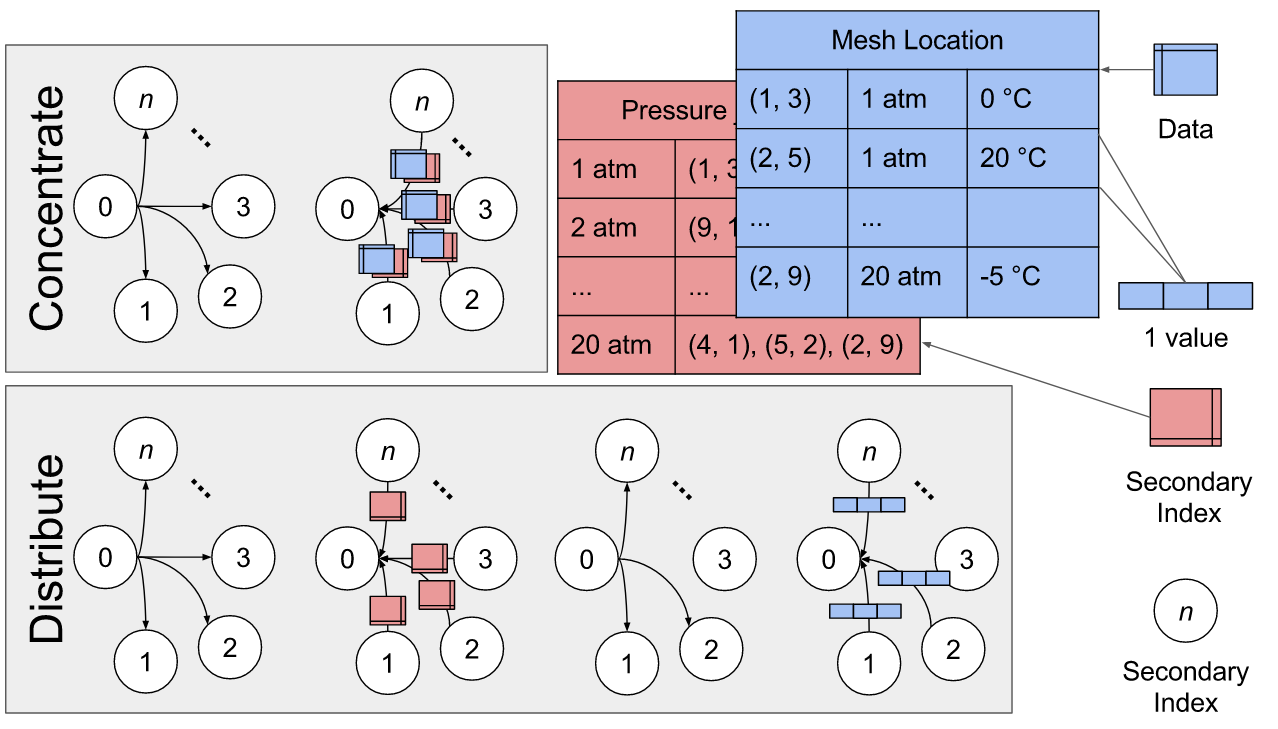
\includegraphics[width=19pc,angle=0]{figures/example.png}\\
  \caption{For a multi-part query with locality, migrating for distribution
  (solution 1) takes more RPCs while migrating for concentration (solution 2)
  risks of overloading the client.}
  \label{fig:example}
\end{figure}


